\Chapter{Language-augmented multi-agent learning}{Learning to communicate with a pre-defined, discrete language}

\label{ChapterComm} 

\section{Introduction}

% FIGURE communication with emergent language vs pre-defined: "we want to show how we can teach language to agents, and what benefits it gives. while there is a cost to pay for teaching langugage to agents, the benefits are great"

% Context
Multi-agent deep reinforcement learning (MADRL) aims at learning how to behave in social settings where multiple intelligent agents interact. This social component adds complexity to the learning process, requiring agents to master additional skills to engage in these environments properly. 
One essential skill in such settings is communication, playing a crucial role in facilitating social interactions. It is observed in various forms across many social animal species~\citep{Smith2003_AnimalSignals, Searcy2010_AnimalCommEvo}, and of course, humans, where it enables a great range of social abilities from sharing information about local observations to negotiation, knowledge transmission, and teaching~\citep{Greene2003_Communication}. 
Taking inspiration from these natural systems, groups of artificial agents can certainly benefit from being able to communicate with partners for sharing information gathered locally and expressing their intentions. 

% Differentiable emergent communication
As described in Section~\ref{sec:MADRL:EmergentCommunication}, learning to communicate accounts to learning (i) \textit{what information to transmit} and (ii) \textit{how to transmit it}. A solution provided by MADRL is \textbf{differentiable emergent communication}, where agents develop communication protocols from scratch driven mainly by the goal of maximising returns. Using differentiable neural networks to produce messages allows learning communication as a sub-module of the policy through gradient back-propagation of the RL objective~\citep{Zhu2024_MACSurvey}. In other words, the problem of learning (i) and (ii) is entirely entrusted to the deep RL algorithm. Whether this approach could lead to the emergence of a language is itself debatable~\citep{Lazaridou2020_DeepEmergentComm, Galke2022_Emergent}. Some approaches try to improve emergent communication in this regard, as we will see in Section~\ref{sec:LAMAC:RW_LanguageDef}. However, in MADRL research, this problem is usually disregarded to focus on how communication improves performance. 

% Problem with DEC
However, this approach suffers from significant drawbacks. One important issue is the \textbf{lack of interpretability} of the emerging communication systems. Since multi-agent systems are targeted toward applications in human-populated environments, interpretability becomes an important matter~\citep{Mikolov2018_RoadmapMachineIntell}. If provided, it would enable transparent human-agent interactions and offer tools for evaluating the reasoning of learnt artificial agents. Researchers have proposed techniques to analyse the resulting communication processes by clustering messages based on state-message correlation~\citep{Lin2021_GroundMAC, Tucker2021_DiscreteEC, Li2022_EmDicrComm, Karten2023_InterpretEmComm}, identifying patterns in emergent languages~\citep{Havrylov2017_EmergenceLang}, or mapping emergent languages to known entities~\citep{Kottur2017_NaturLangEmerg}. These approaches require tedious analysis of the emergent languages, offer no guarantees of success, and need to be applied separately to each independently trained group of agents, as each one develops its own unique communication protocol. 
Another approach is to bias the emerging communication protocols to carry meaning related to external modalities (e.g., visual inputs, actions, real-world concepts). These grounding approaches, reviewed in Section~\ref{sec:LAMAC:RW_Grouding}, guide emergent communication by informing potential useful meanings to convey in the communicated messages. However, this does not solve the interpretability issue, as emergent languages still require some post hoc analysis to be, still imperfectly, interpreted~\citep{Lin2021_GroundMAC, Tucker2021_DiscreteEC}. 

% Advantages of natural languages
A suitable solution to the interpretation issue would be to \textbf{have agents converse using a language} understood by humans. 
Rather than trusting the agents to develop a functioning communication system on their own, teaching them a pre-defined (as opposed to "emergent") language would have many benefits. 
Natural languages have evolved into very efficient communication systems, enabling the vast range of social interactions we take part in. Language allows describing parts of our environments to share local information with others. It allows expressing needs to explain intentions, negotiate, or ask for help. As a shared tool for expressing meanings, it supports the development of culture and the transmission of knowledge. 
In addition, language has been shown to play an important role in the intellectual development of children~\citep{Vygotsky1934, Tomasello2009_Cultural}. This idea has motivated research on language-augmented learning, reviewed in Section~\ref{sec:LAMAC:RW_LARL}, to study how language can be used to guide the learning of artificial agents. 
Overall, providing a language to agents is a way to guide training by introducing a bias on how the environment should be understood and how communication should be conducted. If done successfully, the resulting language-augmented agents would be easier to evaluate, interact and bond with~\citep{Crandall2018_CoopWithMachines, Mikolov2018_RoadmapMachineIntell, Liu2022_ChildChatbotReading}. 

% Chapter objective
While some previous works have experimented with language-based communication, to the best of our knowledge, no study applied it to embodied multi-agent environments. Indeed, learning to communicate with a pre-defined language to solve an embodied task presents its own challenges. It requires a reliable source of language examples and an algorithm capable of learning a language without interfering with policy learning. In this chapter, we propose a solution to these issues by training MADRL agents to produce language utterances that describe their observations. 
The learning algorithm, detailed in Section~\ref{sec:LAMAC:Method}, trains agents to solve the multi-agent task while grounding their observations in language examples. This serves a double purpose: (i) \textbf{enabling agents to learn language-based communication}, while (ii) \textbf{guiding representation learning} by providing an efficient way of extracting valuable information from the world. To allow this, we provide agents with language examples that show how the pre-defined language should be used to describe observations. This data is used to train supervised language objectives concurrently to training on the multi-agent RL objective.  

Through a series of experiments, we show that the cost we pay to train language-augmented agents is easily justified by the advantages brought by language. We demonstrate that language-based communication is easier to learn and more efficient than emergent communication baselines, as the pre-defined language is made to compress the informational content of observations to fit the needs of the task at hand. Having agents communicate with language also enables interesting capacities, namely:
\begin{itemize}
    \item \textbf{better generalisation} of experience to changes in the environment,
    \item \textbf{better adaptation} to new partners,
    \item and easy \textbf{interactions} between humans and the learnt agents.
\end{itemize}
Crucially, language guidance helps agents structure their understanding of the world with linguistic concepts, resulting in faster learning. 


% TABLE advantages of communicating with language
% \begin{table}[]
%     \begin{tabular}{cccc}
%     \hline
%                     & Emergent-Continuous & Emergent-Discrete & Language \\ \hline
%     Training scheme & \begin{tabular}[c]{@{}c@{}}RL from task reward \\ (+ Grounding)\end{tabular} & \begin{tabular}[c]{@{}c@{}}RL from task reward \\ (+ Grounding)\end{tabular} & Supervised \\
%     Bandwidth & High & Low & Low \\
%     \begin{tabular}[c]{@{}c@{}}Interpretability\\ \& Interaction\end{tabular} & Very difficult & Difficult & Straightforward \\ \hline
%     \end{tabular}
%     \caption{Comparison of different communication learning paradigms: emergent communication with either continuous (Emergent-Continuous) or discrete (Emergent-Discrete) signals, and language-based communication (Language). The training approach for emergent communication is mainly based on RL, with the possibility of adding some grounding, while language is learnt with supervision. The bandwidth of continuous signals is very high, while the discrete symbols of Emergent-Discrete and Language allow more compression. Finally, Language allows straightforward interpretation of communication acts and interaction with agents, while both interpretability and interaction are difficult with emergent discrete language, and even more complex with continuous signals that can take an infinite number of different values.}
%     \label{tab:LAMAC:CommStrats}
% \end{table}





% -------------------------------------------------------------------------------------------------

\section{Language and Communication in Artificial Intelligence: Related Works}\label{sec:LAMAC_RW} 

\subsection{Language and Emergent Communication}\label{sec:LAMAC:RW_LanguageDef}

% What's a language
A language can be defined as a shared set of conventions for expressing meaning~\citep{Pinker1990_NaturalLang, Steels1995_SelfOrgVoc}. In natural languages -- i.e., languages that emerged naturally in human cultures --, large vocabularies and complex grammar systems form a rich sets of shared conventions allowing humans to communicate about a large variety of different matters. This is permitted by two key properties of these languages. First, natural languages are combinatorial. They use basic building blocks (e.g., phonemes, syllables) and combine them to construct rich semantic constructs that can hold complex meanings~\citep{Zuidema2018_Combinatorial}. Second, they are compositional: the meaning of a combination of language blocks is a function of the meaning of the combined blocks~\citep{Smith2003_CompoEmerg}. These properties allow natural languages to express a seemingly infinite number of different meanings from a finite set of different symbols. Importantly, they allow to compress information to ensure less costly communication acts and simpler language transmission~\citep{Sigurd2004_ZipfRevisit, Gibson2019_EfficiencyShapeLang}. As a result, natural languages have been shown to have a nearly optimal expressiveness to compression ratio~\citep{Kirby2015_CompressionComm, Gibson2019_EfficiencyShapeLang}, ensuring high efficiency of communication acts and making these languages easier to learn~\citep{Carr2016_CulturalEvoLang}. 

    Experiments involving emergent communication were initially aimed at studying how such languages emerge and evolve in populations of independent agents~\citep{Steels1995_SelfOrgVoc, Nowak1999_LanguageEvo, Vogt2005_EmergenceCompo, Brighton2005_LanguageAsEvo, Kirby2015_CompressionComm}. These experiments showed that languages are cultural adaptive processes that evolve through their numerous independent uses~\citep{Steels1995_SelfOrgVoc, Kirby2015_CompressionComm, Christiansen2008_BrainShapeLang}, and are shaped by environmental~\citep{Perfors2014_WorldShapeLang} and physiological~\citep{Christiansen2008_BrainShapeLang} constraints. Iterated learning experiments studied the transmission of language between successive generations of language users~\citep{Smith2003_IteratedLearning, Vogt2005_EmergenceCompo, Kirby2015_CompressionComm}. They revealed that learning from a limited set of language acts results in a transmission bottleneck ultimately favouring combinatorial and compositional structures in languages. In this context, differential emergent communication has also been used to extend the study of language evolution to the multi-agent reinforcement learning setting~\citep{Havrylov2017_EmergenceLang, Kottur2017_NaturLangEmerg, Lazaridou2017_EmergNaturalLang, Chaabouni2019_AntiEfficient, Rita2022_PopHetero}. To this end, it has an interesting potential for studying the impact of embodied learning on the evolution of language~\citep{VanEecke2022_LangGameMARL}.

However, in the MADRL context, emergent communication, in its differentiable form, has been re-purposed as a tool for optimising multi-agent policies~\citep{Zhu2024_MACSurvey}. In this new task-oriented setting, the emergence of language properties is disregarded to focus on performance on a given multi-agent task. Differentiable communication fits well in the neural paradigm of deep RL, allowing end-to-end learning of communication mechanisms without supervision~\citep{Foerster2016_DIAL, Sukhbaatar2016_CommNet, Mordatch2018_GroundedCompo, Jiang2018_ATOC, Jaques2019_SocialInfluence, Singh2019_IC3Net, Das2019_TarMAC, Kim2018_SchedNet, Zhang2019_VBC, Han2023_MBC}. But, while emergent communication is almost always shown to be effective (i.e., improving performance), multiple works have highlighted its important limitations for this new purpose~\citep{Kottur2017_NaturLangEmerg, Lazaridou2020_DeepEmergentComm}. Emergent languages trained only from return maximisation lack the advantageous qualities of natural languages, namely compositionality~\citep{Galke2022_Emergent}, compression~\citep{Chaabouni2019_AntiEfficient}, and consistency of used signals~\citep{Kottur2017_NaturLangEmerg}. 
\citet{Bouchacourt2018_HowAgentsSee} also showed that agents trained with differentiable communication are able to successfully communicate about noisy inputs. This shows that they have not learnt to communicate about underlying concepts present in their input data, but rather land on an arbitrary consensus on how to represent their observations. 

These issues demonstrate that learning emergent communication only from communication success does not result in structured languages. However, by refining the training process, emergent languages can recover some qualities of natural languages. For example, compositionality can be improved by constraining the size of the vocabulary~\citep{Mordatch2018_GroundedCompo} or increasing the size of the population~\citep{Chaabouni2022_EmCommScale, Rita2022_PopHetero}. Consistency of used signals can also be improved by maximising the mutual information between the input data and the generated messages~\citep{Eccles2019_EmCommBiases}. 

These numerous works on emergent communication help us identify the important qualities of natural language and how they enable efficient communication. They show that emergent languages can be driven to emulate these qualities, provided the right experimental designs and algorithmic choices. Crucially, they show that communication performance does not necessarily imply communication efficiency and, thus, that learning emergent communication from return maximisation alone produces poor communication mechanisms.  




\subsection{Improving Emergent Communication with Grounding}\label{sec:LAMAC:RW_Grouding}

% Grounding definition
Previously cited issues of differentiable emergent communication may be all connected to a more fundamental problem: a lack of conceptual content in communicated signals. This can be related to the \textbf{symbol grounding problem}, defined by \citet{Harnad1990_SymbolGrounding} as the problem of associating meaning from the environment to a priori meaningless symbols. In natural languages, words and sentences carry meaning that is independent of the language itself: e.g., the symbol "apple" encodes a meaning that does not depend on the English language to exist. This consensus on how to express universally recognised meanings allows effective communication about these meanings. In the language evolution domain, the problem of grounding is crucial to understand how humans learn and use language~\citep{Siskind1992_LangAcquis, Brent2001_VocDev}, and how languages can emerge from grounded linguistic interactions~\citep{Steels2000_AIBO, Vogt2002_PhysicalGrounding, Steels2015_TalkingHeads, Nevens2020_ConceptLearn, Botoko2024_LingConvent}. 

% DEC lacking grounding
In Section~\ref{sec:MADRL:EmergentCommunication}, we defined differentiable emergent communication as learning a differentiable sub-step of the agent's policy to maximise the obtained returns. This training process does not have any requirement on how communication actually occurs: if it carries any information, if messages have any impact on the receivers, or if it has any kind of structure. While we can expect agents to learn to communicate about their observations, learning only from RL feedback gives no guarantee of this~\citep{Lowe2019_Pitfalls}. Indeed, we expect agents to learn to extract meaningful concepts from their input data, with only task performance as guidance. This is probably too much to expect. As shown by \citet{Bouchacourt2018_HowAgentsSee}, a more probable outcome is that agents will find an arbitrary consensus on how to communicate about observations, without actually using any concepts that appear meaningful to us. This may be one source of explanation for the issues cited in the previous section: \textit{how can symbols be combined and composed if they do not carry meaning?} This is also a fundamental problem for interpretation, as trying to understand potentially meaningless utterances would be pointless. 

% Grounding approaches
Therefore, instead of relying on return maximisation to produce meaningful communication, agents could benefit from explicitly grounding their messages into meaningful concepts. To do so, we can bias the training process by forcing communication to carry meaning related to external modalities. This can be achieved by adding auxiliary learning tasks on which agents are either pre-trained or trained on concurrently to RL training. By external modalities, we mean any source of meaning that is independent of the agents and the task at hand. The environment, and how the agents perceive it, is a source of meaning that can be leveraged to infuse meaning in the information transmitted between agents. By learning to reconstruct the input data from the communicated messages, agents can learn to maximise the informational content about their observations in their messages~\citep{Lowe2020_S2P, Lin2021_GroundMAC, Karten2023_CompoConcept, Karten2023_IMGSMAC}. Another external source of meaning is natural language. When used to describe the environment, it associates important environmental configurations with words and sentences. It also purposefully discards worthless or superfluous information in the input signals by simply not putting words on these. Learning to make these connections, by associating observations with corresponding language descriptions, allows agents to identify key concepts of their input space to communicate about~\citep{Lazaridou2017_EmergNaturalLang, Das2017_CoopVisDial, Havrylov2017_EmergenceLang, Lazaridou2020_MACNatLang, Tucker2021_DiscreteEC}. These grounding approaches are a way to help agents learn meaningful communication with the support of the additional supervised learning objectives. It helps fill the gap of task-oriented RL, by providing guidance for learning to identify concepts.


% In the neural paradigm of differentiable communication, agents starts with a randomly initialised neural network for generating messages. Training this communication policy network with RL drives its parameters to generate messages that improve the obtained returns. However, this training process does not have any requirement on how communication actually occurs: if it carries any information, if messages have any impact of the receivers, or if it has any kind of structure. Thus, this is not a surprise that learning differentiable communication only from a task-oriented RL feedback does not produce efficient languages. 

% This is even more unsurprising when looking back at our definition of differentiable communication: as a differentiable sub-step of the action-selection process. In other words, the message generation function is a sub-function of the policy. But, in this neural paradigm, the policy acts as a black box of which only the input and output are explicitly defined and easily interpretable. Thus, another way of looking at differentiable communication is to see it as probing into this black box: looking at the output of a particular module of the policy. Trying to interpret the meaning of this signal is a matter of explaining the inner reasoning of a neural network, which is a research problem in itself~\citep{Samek2021_ExplainDNN}. 
% While it can be expected that the probed message has some kind of connection to the final output (here the agent's action), understanding the nature of this connection and the informational content of the message is likely to be a difficult task. 



\subsection{Learning Natural Language}\label{sec:LAMAC:RW_NaturalLang}

Taking this to the extreme allows learning to use natural language for communication, by learning to replicate human-generated sentences and generating natural language messages~\citep{Wang2016_LangGameInteract, Das2017_CoopVisDial, Lewis2017_Deal, Agarwal2019_CommunityRegul, Lee2019_CounteringLDrift, Lazaridou2020_MACNatLang, Gupta2021_DynamicPop}. Using natural language instead of emergent communication does not completely solve the problem of learning to communicate. Agents still need to understand what symbol relates to what meaning and how compositional structures describe different environmental configurations. 
But, it solves the problem of interpretability, by making agents converse with the same tools as human experimenters. 

% Learning language requirements
However, learning to use a pre-existing language requires access to demonstrations of this particular language. Thus, to teach natural language to agents, previous works have been restricted to training environments that feature a large amount of language examples. Such environments are usually centred around language, with language being either the agents' observation or action domain. 
For example, the \textit{Lewis signalling games}~\citep{Lewis1969_Convention}, or \textit{language games}~\citep{Steels1995_SelfOrgVoc, Steels2000_AIBO}, usually involve interactions between two agents: one speaker and one listener; where the goal is for the speaker to transmit some information about its observation and for the listener to correctly interpret the incoming message. This framework can be used for describing natural language processing tasks, such as translation~\citep{Lee2018_EmergentTranslation, Lee2019_CounteringLDrift, Lu2020_CounterLangDrift} or image captioning~\citep{Lee2019_CounteringLDrift, Lazaridou2020_MACNatLang, Gupta2021_DynamicPop}, allowing to exploit large datasets of language examples. 
Another example is \textit{visual dialogue}~\citep{Das2017_CoopVisDial, Agarwal2019_CommunityRegul}, which can benefit from datasets of conversation about images to learn communication with natural language.

% Limits of language-centered envs
While these settings show successful instances of learnt language-based communication, they fail to emulate the complete role of language in human communication: as a tool for supporting multi-agent interactions. In language-centred environments, agents lack of embodiment: they are defined only by their language abilities and have no physical interactions independent of the language task. We argue that this limits both:
\begin{itemize}
    \item the complexity of the learning problem: in embodied, multi-agent settings, communication is not necessarily central to the task, agents need to learn when and how to use it best for the task at hand;
    \item the actual language abilities of these agents: physical interactions play an important role in learning language, thus, learning only from language data, even with visual grounding, can result in incomplete knowledge of the meaning behind natural language symbols. 
\end{itemize}
In Section~\ref{sec:LAMAC:Method}, we propose an approach for alleviating these issues, making a step towards learning language in multi-agent robotic settings. 

% LLMs 
Lastly, when it comes to using natural language almost as proficiently as human beings, \textit{large language models} (LLMs) are now widely recognised as the most evident choice. Thanks to their extremely large architectures, extensive pre-training on large amounts of human-generated text, and use of RL to better fit human preferences~\citep{Christiano2017_RLHF, Ouyang2022_InstructGPT}, they excel in generating human-like text. With some fine-tuning, they can easily be adapted to work with multi-modal inputs, allowing to handle visual and even behavioural modalities~\citep{Driess2023_PaLME}. With specific prompting techniques, LLMs can be driven to exhibit particular behaviours and even adopt personas~\citep{Li2023_CAMEL, Park2023_LLMtown, Perez2024_CulturalEvo}.
All these features allow to define \textit{agent-based LLMs}~\citep{Li2023_ToMLLM, Liu2024_HLA, Zhang2024_CoELA} for studying multi-agent settings with LLMs mimicking human reasoning. 
There is no doubt that these capabilities have an interesting potential for handling more complex multi-agent tasks and interacting with artificial agents. 
However, there are still some issues and limitations preventing the wide adoption of LLMs. Their extremely high pre-training and fine-tuning costs prevent their adaptation to specific settings. 
While using LLMs "out-of-the-box" as a human-like language module can enable general language capacities, this inevitably means that the language-learning phase is lost. One goal of this work is to demonstrate that the act of learning the language can guide the agents in learning how to behave in their environment. In the next section and later in the experiments (see Section~\ref{sec:LAMAC:Experiments}), we provide arguments and experimental results to back this claim. 







\subsection{Language-Augmented Learning}\label{sec:LAMAC:RW_LARL}

An important idea at the core of this work is the fact that language supports learning and intellectual development. In developmental psychology,~\citet{Vygotsky1934} has shown the central role of language and language-based social interactions in the intellectual development of children. Language serves structured reasoning as a way to describe the learning environment, set goals based on previously experienced or observed interactions, imagine new goals based on the composition of known, language-expressed goals, and internalise social interactions for supporting later goal-based learning~\citep{Vygotsky1934, Piaget1952, Tomasello2009_Cultural, Lupyan2012_WhatWordsDo}. 
 % the acquisition of knowledge

Following these observations, researchers have explored different ways by which language can guide the training of RL agents. Language can be used to ground the agents' understanding of their environment, by learning to describe observed situations~\citep{Ruis2020_gSCAN, Hanjie2021_EMMA, Hill2021_Grounded}. This allows efficient representation learning and better generalisation to unseen environmental configurations and even different domains with similar entities~\citep{Narasimhan2018_Transfer}.
Describing the world with language can also enable the prediction of future outcomes~\citep{Huang2022_InnerMonol, Lin2023_Dynalang, Nottingham2023_DECKARD}, allowing language-grounded model-based RL. 
Like with human beings, language can be used to express goals~\citep{Lynch2021_MCIL}. By expressing goals with language, agents can learn to associate the experienced trajectories with the linguistic concepts in the observed goals. In such goal-directed learning settings, language models can be used to generate rewards to guide training~\citep{Carta2022_EAGER}. This can make the learning of new goals easier~\citep{CoReyes2018_GPL, Shridhar2021_CLIPort, Li2022_LID} and even enable agents to imagine new goals by themselves using the learnt structures of language~\citep{Colas2020_Imagine, Akakzia2021_DECSTR, Colas2022_Autotelic}. This can be further implemented into hierarchical RL, with a high-level instruction policy generating language goals and a low-level policy selecting actions to complete these goals~\citep{Hu2019_HierarLang, Jiang2019_CLEVR, Weir2023_HLLP}. 
In this domain, the great language abilities of LLMs are also welcome to describe the agents observations~\citep{Huang2022_InnerMonol, Zhu2024_CognitiveLLMs}, give them instructions~\citep{Ahn2022_SayCan, Huang2022_InnerMonol, Carta2023_GLAM, Huang2023_GroundDec}, provide them with rewards~\citep{Baumli2023_VLRewards}, or even serve as policies conditioned on both visual input and language~\citep{Reed2022_Gato, Brohan2023_RT2, Driess2023_PaLME}.

These numerous applications show the immense potential of language to guide the training of artificial agents. In this work, we aim to show that this is also true in multi-agent settings. In addition to communication, language can help agents acquire a better understanding of their environment and better generalisation abilities for handling dynamic multi-agent settings. 


% LA-Learning
% - language in RL (before LLMs)
% - LLMs: for guiding robotic control, for helping RL
% - VLAs

% Language augmented MARL

% issue in machine learning on how to give general knowledge to artificial intelligence.
% on one side, specialised machine learning models are extremely performant on their task (e.g., LLMs, Computer vision), but are restricted to their task and require extensive training to adapt to new objectives or modalities
% on the other side, embodied RL agents can learn to perform complex tasks in rich environments (e.g., complex games, pixel inputs), but they lack general knowledge about the world and ability to reason about high-level concepts
% Thus, there is a need for ways to transmit general knowledge to RL agents for them to better understand their environment, the entities that populate it, and the rules that govern it. 
% Language can be a tool for giving high-level information to artificial agents

% Apart from these obvious qualities of language, other advantages may exist (cite and see refs of Colas2022):
% - Vygotsky have studied the role of language in the psychological and intellectual development of children, and shown its importance for learning to contruct high level reasoning
% - language allows easy bonding between very different entities (humans from different cultures, humans and animals, human and artificial agents)

% Mirolli2011_VygotskyanRobot
% Tomasello2009_Cultural



% Conclusion ?
% looking back on these works accross different domains of AI, we can summarise and formulate a starting point for this work
% Communication is a crucial element of social interactions
% Differentiable emergent communication has many important limitations, one most critical being the lack of interpretatability that prevents the deployment of learnt communicative agents in human-populated envrionments
% Language offers an efficient communication system, by design, and a learning tool for understanding the environment by learning what environment elements map to important concepts and how different concepts can relate to each other
% Thus, we argue that a promising avenue for MADRL research is to study how language can be learnt in MADRL settings, and how it can be used for helping agents to learn, reason, and communicate efficiently.



% -------------------------------------------------------------------------------------------------

% \section{Background on natural language processing}



% -------------------------------------------------------------------------------------------------

\section{Language-Augmented Multi-Agent Communication: \\Our Method}\label{sec:LAMAC:Method}

\subsection{Problem Statement}

% Our embodied setting
In this section, we describe our approach for learning multi-agent communication with a pre-defined language used for grounding and communication. 
Drawing inspiration from the different bodies of literature reviewed in the previous section, we design an architecture that allows embodied agents to learn a language for describing what they observe. 
Our objective is to show that this approach can help improve learning and communication in classical multi-agent settings.
In such settings, communication is not central to the learning problem. Agents have to perform physical actions to interact with the environment and ultimately complete the task. 
Communication is a tool for influencing the behaviour of other agents. Agents have to learn how and when to use it to maximise their returns. 
With our language-based approach, we aim to demonstrate that language helps both the policy learning problem, by grounding environmental elements and actions in the given language, and the communication learning problem, by providing a known-efficient way of communicating about the world. 
% we want to do this in an embodied setting, which means:
% agents are situated in an environment they can interact with
% they have to interact with it with physical actions to complete the task
% this is crucial: the main objective is to complete a physical task. communication here is a tool to help agents in their multi-agent task
% agents must learn to use communication as a means to optimise their behaviour

% Our assumptions
% To enable agents to communicate about their observations, we need a reliable source of observation-language descriptions examples. 
The objective is to emulate a setting where a group of robots learns to perform a multi-agent task with an oracle, human or machine, that teaches them how to use a given language for the purpose of the task. Thus, during training, we assume that we have access to language descriptions of local observations. In Section~\ref{sec:LAMAC:LanguageDef}, we define the language used in our setting and describe how the language descriptions are generated. Because we aim to train agents for rather simple robotic tasks, we do not need to teach them a complete natural language made for handling a wide variety of human situations. Instead, a simple language is defined with only the required vocabulary and grammar to fit the needs of the task at hand. Importantly, the provided descriptions give no additional information about the environment. They only provide a particular way of representing the meaningful content that is inside the agents' observations. By teaching this specific structured representation system to our agents, we aim to guide them in learning how to understand their observations and how to communicate efficiently about them.
% the lack of embodiment of language-based agents described in section {} is mainly due to a lack of aligned data to learn language in robotic settings
% we want to enable agents to communicate about their observations
% our goal is to emulate the setting of having robots learning a task, with an oracle (human or machine) teaching them how to use a language
% we assume that we have access to language descriptions given by an oracle (at least in the initial training setting): for each local observation, we have a corresponding description
% these descriptions give no additional information about the environment
% but, they provide guidance for representing the content of observations. this is a desired feature: we want to guide the learning process of our agents by showing them what is important and what should be communicated
% because we are in a simple task, we don't need to use natural language, as it would be way too complex for the purpose of our robotic settings
% thus, we will define a much more simple language that serves the communication needs of our setting (see Section )

% to counter the lack of data for learning language in our setting...
% similar to previous works {Wang2016_LangGameInteract, (voir LARL works)}, we build a parser that produces language utterances




\subsection{Agent Architecture}\label{sec:LAMAC:Archi}

% Overall algorithm
To enable learning language-based communication in a multi-agent setting, we augment MADRL agents to equip them with language capabilities. We define a learning algorithm that fits in the CTDE paradigm: 
\begin{itemize}
    \item decentralised agents can generate messages and actions from their local observations only;
    \item these agents are trained in a centralised manner to improve the training efficiency of local policies and language modules.
\end{itemize}
Concretely, we build upon the MAPPO algorithm (see Section~\ref{sec:MADRL:CentralCritic};~\cite{Yu2021_MAPPO}): each agent has a local policy for selecting its actions and a centralised value used during training, as shown in Figure~\ref{fig:LAMAC:archi}. 
In addition, the agent architecture is modified to include a communication policy that selects the information to communicate and language modules for generating and understanding language utterances. 

\begin{figure}
    \centering
    % \includesvg[width=0.95\linewidth]{Figures/LAMAC/archi.svg}
    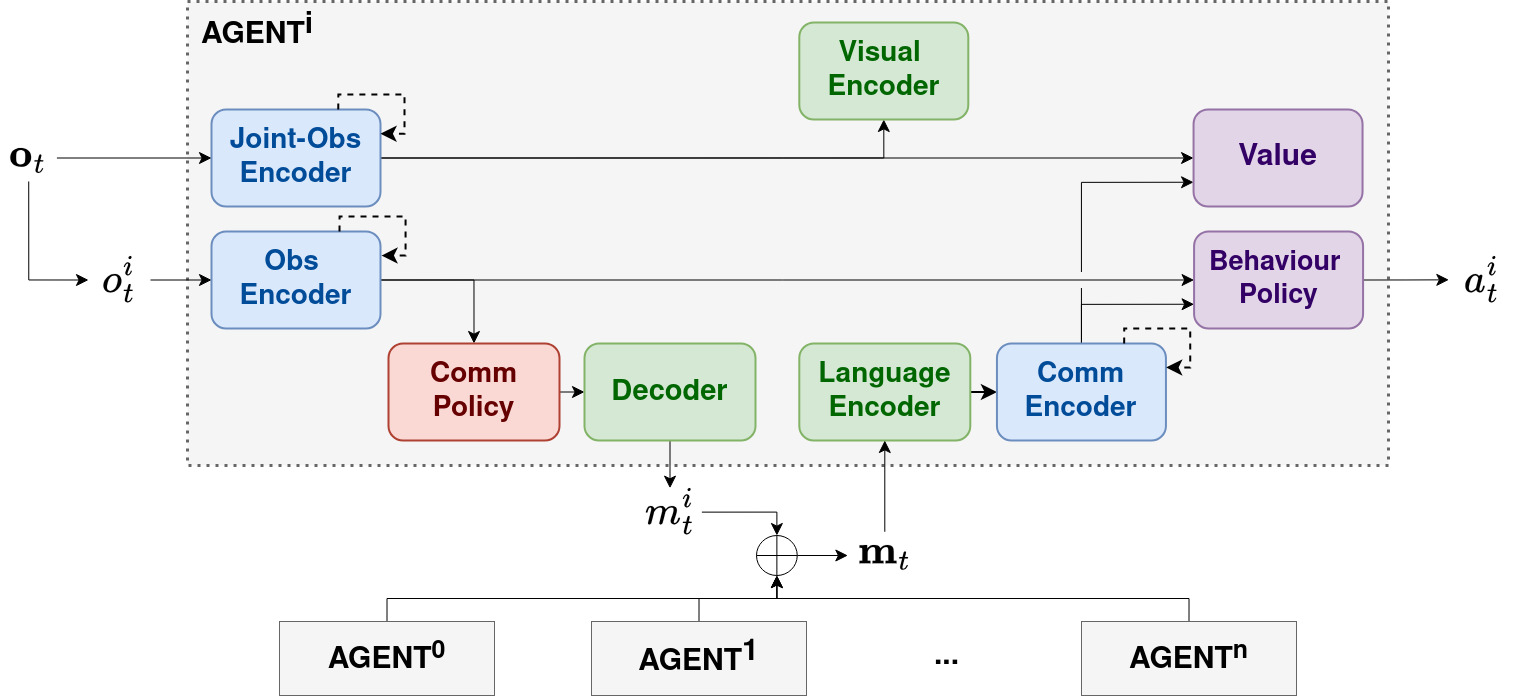
\includegraphics[width=0.95\linewidth]{Figures/LAMAC/archi.jpg}
    \caption{Illustration of the architecture of language-augmented agents. Each module represents a small neural network with a different purpose in the architecture. \textcolor{RoyalBlue}{\textbf{Encoder modules}} receive incoming information (observations or communication) and embed it in latent representation used in further modules, with dashed arrows indicating that they contain a recurrent neural network to enable having memory of previous steps. The \textcolor{BrickRed}{\textbf{communication policy}} selects what information in the observation should be communicated. \textcolor{ForestGreen}{\textbf{Language modules}} provide language capabilities: the decoder generates messages, the language encoder transforms incoming messages in a compact numerical representation, and the visual encoder is there for training the language encoder (as described in Section~\ref{sec:LAMAC:CLIP}). Finally, \textcolor{Plum}{\textbf{RL modules}} take information from both observations and communication to select actions.}
    \label{fig:LAMAC:archi}
\end{figure}

% FIGURE ? Learning signals 

\subsubsection{Decentralised Action-Selection}

At each time step $t$, agents start by receiving their local observation $o^i_t$, which is fed to the \textit{observation encoder} $\mathrm{E}^i_{obs}$. It produces an observation embedding: $\mathrm{E}^i_{obs,t}(h^i_{o,t})=c^i_{obs,t}\in\R^H$, with $E$ the embedding dimension and $h^i_{o,t}=(o^i_0,...,o^i_{t-1})$ the observation history of agent $i$. Here, agents have access to their observation history because the encoder is defined as a recurrent neural network, allowing them to memorise some information from previous steps (see Appendix~\ref{app:LAMAC:archi} for a detailed definition of the neural networks in each module). The observation embedding then goes to the \textit{communication policy} $\pi_{comm}^i$ to produce the communication context: $\pi_{comm}^i(c^i_{obs,t})=c^i_{comm,t}\in\R^C$, with $C$ the context dimension. This communication vector $c^i_{comm, t}$ is a latent representation of what the agent wants to communicate to its partners. It goes through the \textit{language decoder} $\mathrm{D}^i$ to generate a message, as described later in Section~\ref{sec:LAMAC:Captioning}: $\mathrm{D}^i(c^i_{comm, t})=m^i_t\in L$, with $L$ the set of all possible sentences in our language. The generated message is then sent to other agents via the communication channel described below. After exchanging messages, the incoming message $\mathbf{m}_t$ goes through the \textit{language encoder} $\mathrm{L}^i$ to encode the message into a vector representation, as described in Section~\ref{sec:LAMAC:CLIP}, which itself is fed to the \textit{communication encoder} $\mathrm{E}^i_{comm}$ to produce the social context: $\mathrm{E}^i_{comm}(\mathrm{L}^i(\mathbf{m}_t))=c^i_{soc, t}\in\R^C$. Note that the communication encoder is also defined as a recurrent neural network to allow keeping some memory of previous messages. Finally, the social context is concatenated to the observation embedding to construct the input of the behaviour policy $\pi^i$, which generates the agent's action: $\pi^i(c^i_{obs,t}, c^i_{soc,t})=a^i_t$. 



\subsubsection{Communication Channel}

For exchanging messages, we choose to stick with a rather simple solution where messages are sent to all agents of the system. Thus, after all agents have generated their message, the individual messages are gathered and concatenated to form the broadcast message $\mathbf{m}_t=\{m_t^0,...,m_t^n\}$ that all agents receive. 
This broadcasting approach fits well the kind of settings we are interested in: cooperative tasks with a relatively small number of agents. In such settings, there is no benefit to keeping some information from other agents and we can assume that all agents can be connected by a common communication channel. However, this could easily be adapted to environments with restricted communication channels. For example, we could define a communication range that limits the distance by which agents can send messages to other agents. 


\subsubsection{Centralised Actor-Critic Learning}

In MAPPO, agents learn a centralised value function to guide the training of their decentralised policy. The value function is said to be "centralised" because it takes the joint-observation as input. Using this centralised information during training helps the value function making better value estimation. In our case, the value module takes as input the output of the \textit{joint-observation encoder} $\mathrm{E}^i_{joint,t}(\mathbf{h}_{o,t})=c^i_{joint,t}\in\R^H$, with $\mathbf{h}_{o,t}$ the joint-observation history; and the social context $c_{soc,t}^i$ coming from the communication step. These two vectors are concatenated and through a neural network to generate the value estimate for the current state $V^i(c^i_{joint,t},c^i_{obs,t})\in\R$. This value is used during training to compute the loss of PPO described in Section~\ref{sec:DRL:PPO}. 
% In MAPPO, each agent learns a centralised value function that guides the training of the decentralised policy
% To learn better value estimates, the value function uses information collected by all agents
% In our case, the value function takes as input the history of joint observations and messages
% Thus, each agent has a joint observation encoder that produces a vector $c_jo$
% This vector is then concatenated to the social context to form the input of the value function
% ? PPO losses ?



\subsection{Language Learning}\label{sec:LAMAC:LangLearning}

To enable agents to use a pre-defined language for sharing information, agents must be able to understand the given language and generate language utterances. To learn these two skills, techniques from the domain of natural language processing can be applied. Here, we define the two supervised learning objectives used for training the \textbf{language encoder} and the \textbf{decoder}. 


\subsubsection{Grounding Language Understanding with Contrastive Learning}\label{sec:LAMAC:CLIP}

To understand a given language, one solution is to learn to associate language examples with their meaning as presented in a different data space. Say we have a set of observations $O$ and a set of language descriptions $L$, with one language description $l^i$ for each observation $o^i$. Language descriptions provide a semantic proposal for describing the informational content of observations. To learn how this language works for extracting and arranging meaning, we can learn to associate observation-description pairs together and dissociate the non-paired elements. This is the idea behind \textbf{contrastive learning}, that learns relations between different data spaces by learning to associate paired data points~\citep{Oord2018_Contrastive, Tian2020_Contrastive}. We follow the method \textbf{CLIP} (contrastive language-image pre-training;~\cite{Radford2021_CLIP}) that trains two encoders, one for language descriptions and one for observations, both generating compact vector representations of the input. To ground language learning, the encoders are trained to generate representations of observations and descriptions that maximise the mutual information between correct pairs $(o^i, l^i)$ and minimise the mutual information of incorrect pairs $(o^i, l^j)$. Concretely, the \textit{visual encoder} $\mathrm{V}:O\rightarrow\R^C$ and \textit{language encoder} $\mathrm{L}:L\rightarrow\R^C$ are trained to maximise the cosine similarity of correct pairs:
\begin{equation}
    \max_{\theta_\mathrm{V},\theta_\mathrm{L}}\left[cosim(\mathrm{V}(o^i),\mathrm{L}(l^i))\right],
\end{equation}
and minimise it for incorrect ones: 
\begin{equation}
    \min_{\theta_\mathrm{V},\theta_\mathrm{L}}\left[cosim(\mathrm{V}(o^i),\mathrm{L}(l^j))\right],
\end{equation}
with any $i,j\setminus i\neq j$, $\theta_\mathrm{V}$ and $\theta_\mathrm{L}$ the parameters of the visual and language encoders respectively, and the cosine similarity of two vectors: $cosim(a,b)\coloneq\frac{a\cdot b}{\parallel a\parallel\parallel b\parallel}$. Overall, the objective of CLIP can be formulated as minimising the following loss:
\begin{gather}
    L^{CLIP}(\theta_\mathrm{V},\theta_\mathrm{L})=\sum_{i,j}CLIP(i,j),\\
    CLIP(i,j)=
    \begin{cases}
        -cosim(\mathrm{V}(o^i),\mathrm{L}(l^i)) & \text{ if }i=j, \\
        cosim(\mathrm{V}(o^i),\mathrm{L}(l^j)) & \text{ if }i\neq j.
    \end{cases}
    \label{eq:LAMAC:CLIP}
\end{gather}
%This technique allows to learn language by grounding it into the external meaning given by the observation space. 

% Encoding language
To model the two encoders, we use different kinds of neural network architectures. The visual encoder $\mathrm{V}$ can be modelled as a simple MLP (see Section~\ref{sec:NN:DeepLearning}) that transforms an observation vector $o^i\in\R^N$, with $N$ the dimension of the observation space, into the observation embedding $\mathrm{V}(o^i)\in\R^C$. For the language encoder $\mathrm{L}$, we need a more complex architecture as a language description $l^i$ is made of a sequence of tokens: $l^i=(t_0,...,t_K)$, with each token $t_k\in\R^{D^V}$ being drawn from a vocabulary $V$ of size $D^V$, and represented as a one-hot vector. In natural language processing, tokens are the basic blocks of language sequences: e.g., characters, syllables, words, or punctuation marks. To encode a sequence of tokens, $\mathrm{L}$ must be defined as a recurrent neural network, in our case a GRU (see Section~\ref{sec:NN:RNN}). Each token in $l^i$ is successively passed through the GRU: $f_{GRU}(h_k, t_k)=h_{k+1}$, with $h$ the hidden state of the GRU ($h_0$ being initialised with zeros). After all tokens have been handled, the final hidden state $h_K$ is passed through a single neural network layer to output the description embedding $\mathrm{L}(l^i)\in\R^C$. 



\subsubsection{Generating Language by Learning Captioning}\label{sec:LAMAC:Captioning}

To learn how to generate language, we use a second supervised learning task from natural language processing. We adapt the \textbf{image captioning} task that trains a model to generate the language descriptions of images, by feeding it a large number of image-description pairs. In our case, we want the agents to learn to describe their observations. Thus, agents are equipped with a \textit{decoder} $\mathrm{D}:O\rightarrow L$. Given a set of training examples $(o^i, l^i)$, the decoder takes $o^i$ as input and is tasked to generate the corresponding language description $l^i\in L$. 

Similar to the language encoder, the decoder needs a recurrent architecture to generate language utterances. Thus, the decoder will use a GRU that takes as input a hidden state $h_k$ and a token $t_k$, and outputs the token $t_{k+1}$ that follows in the sequence. To generate a single utterance $l^i=(t_0,...,t_K)$, the observation $o^i$ is passed through a neural network to produce a compact representation that can be passed to the decoder as its initial hidden state: $f_{in}(o^i)=h_0$, with $f_{in}:O\rightarrow\R^H$ an MLP and $H$ the dimension of the decoder's hidden state. The GRU then takes as input $h_0$ and a special "start-of-sequence" token $t_0=\text{<SOS>}$, and outputs the new hidden state and following token: $f_{GRU}(h_0, t_0)=(h_1, t_1)$. The process continues until the GRU produces the special "end-of-sequence" token $t_K=\text{<EOS>}$. To learn the captioning task, for each training pairs $(o^i, l^i)$, the decoder generates a candidate sequence $\hat{l}^i=(\hat{t}_0,...,\hat{t}_K)$ and is trained to minimise the cross-entropy: 
\begin{equation}
    L^{capt}(l^i,\hat{l}^i,\theta_\mathrm{D})=-\sum_{k=1}^Kp(t_k)\log\hat{p}(t_k),
    \label{eq:LAMAC:Captioning}
\end{equation}
with $p$ the target probability density and $\hat{p}$ the probability density generated by $f_{GRU}$ from which $\hat{t}_k$ is sampled. 


\subsubsection{Integrating Language Modules}

With these two natural language approaches, we can enable the agents to generate messages that describe their observations and encode incoming messages into embeddings grounded in their observation space. 
To integrate these capacities in the agent architecture, we include three required language modules (depicted in green in Figure~\ref{fig:LAMAC:archi}). They are placed in the agent architecture to allow agents to learn the objectives of CLIP and the captioning task. 

The decoder is placed after the communication policy to generate messages. The input network $f_{in}$ described previously is replaced by the observation encoder and communication policy. Thus, the observation encoder, the communication policy, and the decoder are trained jointly on the captioning task to generate accurate descriptions of the observation. 

Because the language encoder is tasked to encode broadcast messages -- i.e., descriptions of all local observations combined -- it seems adequate to place the visual encoder after the joint-observation encoder. This way, the contrastive learning objective is learnt with centralised information as input of both encoders. 

The data required for training on these objectives is gathered by the agents as they interact with the environment: at each time step, an observation-description pair is gathered by each agent. When the agents' policies are trained, we compute the losses for PPO, CLIP, and the captioning task, and optimise the three together by minimising:
\begin{equation}
    L^{TOT}=\beta_{PPO}L^{PPO}+\beta_{CLIP}L^{CLIP}+\beta_{capt}L^{capt},
    \label{eq:LAMAC:Loss}
\end{equation}
with $L^{PPO}$ defined in Equation~\ref{eq:PPOloss}, $L^{CLIP}$ and $L^{capt}$ defined above, and parameters $\beta$ for weighting each loss (see Section~\ref{sec:LAMAC:DynaWeightLoss} for details on how they are defined).  

This training procedure allows training the agents' policy and language skills completely end-to-end. Note that with the proposed architecture, both the observation and joint-observation encoders contribute to the language losses. Therefore, both the policy and value sides of the agents will be grounded in language, with the input encoders learning to extract language-based concepts from the observations. 





% Mercredi

% -------------------------------------------------------------------------------------------------

\section{Implementation}

\subsection{Language and Oracle Definition}\label{sec:LAMAC:LanguageDef}

To enable agents to communicate about their observations, we define a simple language that allows describing elements from the environments that are important for the task at hand. In this work, we focus on the Predator-Prey setting, where agents need to find preys and coordinate to catch them (see Section~\ref{sec:LAMAC:Exp_Training} for details on the scenario). As agents have a limited field of view, sharing the positions of observed preys to the group should improve the catching speed. Therefore, we design a language that allows this by stating the cardinal position (i.e., "North", "South", "East", "West", and "Center") of the observed preys, as shown in Figure~\ref{fig:LAMAC:oracle}. The \textbf{oracle} is a rule-based program that takes local observations as input and generates the corresponding language descriptions. The resulting language has the following limited vocabulary:
\begin{center}
    $V=\left\{\text{Prey, North, South, East, West, Center}\right\}$
\end{center}
By describing the positions of two preys at most, it can produce descriptions of six tokens maximum (e.g., "Prey North East Prey South West"). 

Despite its apparent simplicity, this language provides the tools for efficiently signalling the region of the grid that other agents should head towards. It is compositional, with the "Prey" token providing structure in sentences -- i.e., after "Prey" always comes a localisation --, and the cardinal tokens that can be composed to express different regions. Importantly, it offers a structured, condensed representation of the agent's observation. This provides the language guidance we sought for understanding the environment. By learning the observation captioning task, the agents will learn to recognise important features in the observations and represent them efficiently.  

\begin{figure}
    \centering
    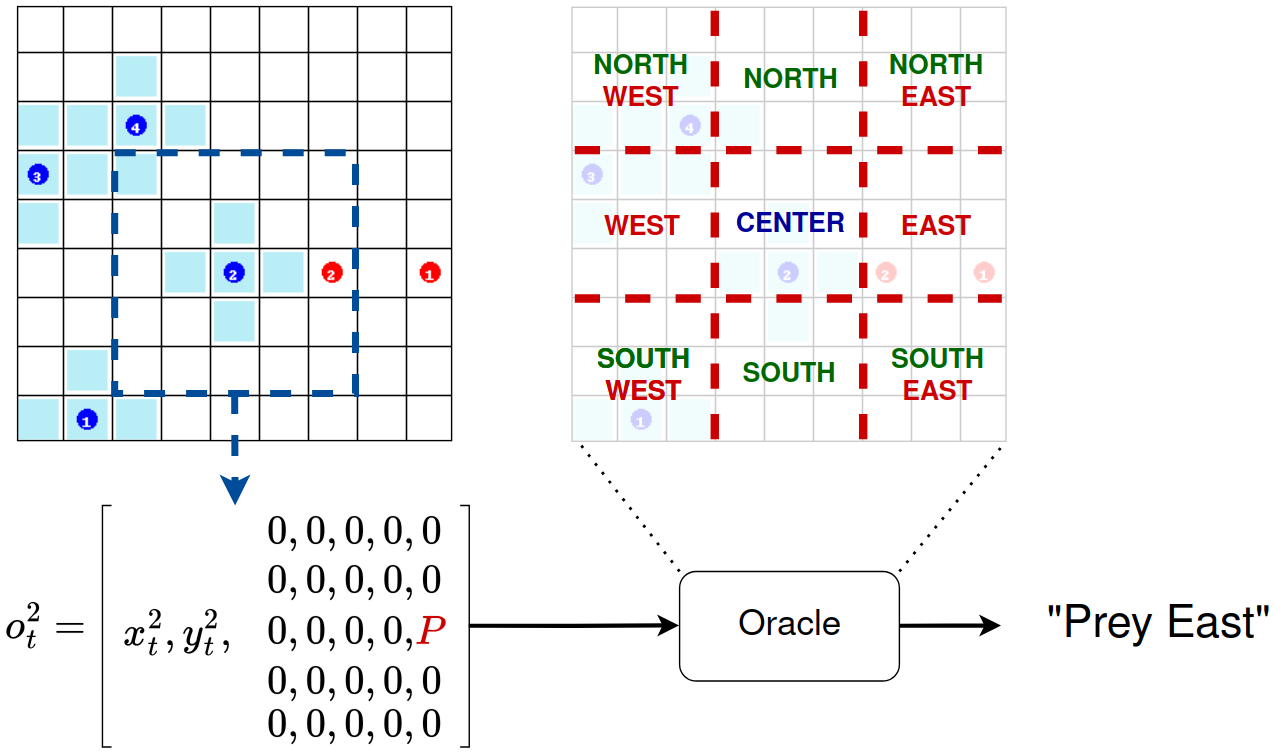
\includegraphics[width=0.8\linewidth]{Figures/LAMAC/parsing.png}
    \caption{Illustration of the oracle's process for describing observations. In the top-left part is a screenshot of the \textit{ma-gym} environment in the Predator-Prey task (agents in blue and preys in red). Agents observe their absolute position in the grid and the objects in their surrounding $5\times 5$ observation range (shown in dark blue). The oracle generates a language description that describes the cardinal position of each observed prey.}
    \label{fig:LAMAC:oracle}
\end{figure}




\subsection{Baselines Definition}\label{sec:LAMAC:BaselineDef}

To try to measure the benefits of learning to communicate with a pre-defined language, we compare the language-augmented agents with four other communication strategies. Here, we define the five compared agent versions:
\begin{itemize}
    \item \texttt{Language} agents use our proposed method for learning to communicate with the pre-defined language. They learn to describe their observations and use the generated descriptions as messages during the episodes. 
    \item \texttt{Oracle} agents use the descriptions given by the oracle as messages. They learn the language tasks as well but do not use the generated messages and instead directly send the oracle's description. They provide a baseline for measuring the impact of RL training on language generation in the \texttt{Language} agents. 
    \item \texttt{Emergent-Discrete} agents learn differentiable emergent communication, with discrete symbols. We provide these agents with the same theoretical language capabilities as the language-augmented agents: they use the same architecture and can generate sentences of the same length with a vocabulary of the same dimension. Thus, they differ in the fact that they do not learn from the language tasks. Instead, they learn to use their discrete symbols through back-propagation of the RL objective, using the Gumbel-Softmax trick to allow gradients to flow through the sampling operation~\citep{Jang2017_GumbelSoftmax}. 
    \item \texttt{Emergent-Continuous} agents use differentiable emergent communication, with continuous signals. They use the architecture illustrated in Figure~\ref{fig:LAMAC:archi} but with no language modules. The messages are directly generated by the communication policy: $m^i_t=c_{comm,t}^i\in\R^C$, with $C=2$ in this case. Inspired by previous work~\citep{Das2019_TarMAC}, we choose this rather small size for continuous messages that still theoretically allows expressing an infinite number of different meanings. 
    \item \texttt{No Communication} agents do not communicate at all. They are here as a baseline to measure the impact of the different communication approaches.
\end{itemize}

% Definition of baselines
% figure with emergent communication

% TABLE summary of differences of each model (Language, Oracle, No Comm, Em-Cont, Em-Discr)

\subsection{Communication $\varepsilon$-Oracle Strategy}\label{sec:LAMAC:CommEps}

When starting to learn language, agents will inevitably generate bad messages. To prevent this from hindering communication learning, we allow agents to use the oracle's description as messages at first and slowly transition to the generated messages. Thus, communication is ensured to serve its purpose from the beginning of training, allowing the policy to learn to use it accordingly. 

To enable this transition from oracle to generated messages, we devise a "\textit{$\varepsilon$-oracle}" communication strategy (inspired from $\varepsilon$-greedy in Q-learning). At each time-step, agents randomly choose whether to send the oracle's description or the generated message, with probabilities of $p(\text{oracle})=\varepsilon$ and $p(\text{generated})=1-\varepsilon$. The $\varepsilon$ parameter is decayed from 1 to 0 throughout training, following a sigmoid-like decay curve, as illustrated in Figure~\ref{fig:LAMAC:comm_eps}. In Appendix~\ref{app:LAMAC:param_decay}, we define formally the function for decaying $\varepsilon$. The parameter $\sigma$ allows controlling the slope of the decay. In our experiments, we stick with $\sigma=2$ to have a slow transition, but it could be interesting to study the effects of different values of $\sigma$ on communication learning. 

\begin{figure}
    \centering
    \includesvg[width=0.5\linewidth]{Figures/LAMAC/comm_eps.svg}
    \caption{Decay curves of the $\varepsilon$ parameter used in the $\varepsilon$-oracle strategy for learning to communicate with language. The parameter $\sigma$ allows controlling the slope of the decay.}
    \label{fig:LAMAC:comm_eps}
\end{figure}

\subsection{Loss Weighting}\label{sec:LAMAC:DynaWeightLoss}

In Equation~\ref{eq:LAMAC:Loss}, we define the total loss optimised by our algorithm, combining losses from different objectives by summing them together. A problem with this method is that different losses might take values of different orders of magnitude, which can prevent all losses from being optimised at the same rate. This is a well-known problem in the multi-task learning literature, that unfortunately does not have a widely recognised preeminent solution~\citep{Vandenhende2021_MultiTask}. Intuitively, we consider that all losses should be of the same magnitude to ensure that they contribute equally to the total loss. Knowing that all losses evolve at very different rates, and inspired from previous work~\citep{Liu2019_MTAN}, we dynamically update the weighting parameters $\beta_{PPO}$, $\beta_{CLIP}$,  and $\beta_{capt}$ so they all have values close to 1. To do so, during training iteration $k$, we have:
\begin{equation}
    \beta_k=\frac{1}{L_{k-1}},
\end{equation}
for each different loss\footnote{For simplicity, we noted only one parameter $\beta_{PPO}$ for the PPO objective. But, $L^{PPO}$ is itself made of multiple losses, as defined in Section~\ref{sec:DRL:PPO}. In our implementation, we actually have different $\beta$ parameters for the policy and value parts of PPO's loss}. In other words, each loss is normalised by the value of the loss at the last iteration of training. We found that it was a simple solution for weighting many very different losses, that yielded the best results in our case. 

\subsection{Implementation Details}\label{sec:LAMAC:ImpDetails}

In Appendix~\ref{app:LAMAC:archi}, we provide a detailed definition of the agent architecture with the neural networks in each module and the set of hyperparameters used in our experiments. All compared versions of the architecture use the same set of hyperparameters, apart from the context dimension $C$ that is set to $2$ for \texttt{Emergent-Continuous} as previously mentioned, and to $16$ for other variants. 
Our code for the architecture and training is available online\footnote{\url{https://github.com/MToquebiau/Language-Augmented-MADRL}}. 

One important information to point out is the use of embedding layers in the language modules, to learn a specific vector representation of each token in the vocabulary~\citep{Mikolov2013_Embedding}. This is a common technique in natural language processing, to help learn the role of different tokens in the given language and how they can be composed in structured sentences. The embedding layers are shared between the decoder and language encoder and learnt during training with the rest of the architecture. 
% Embedding layers
% PPO tricks
% 

% language parameters shared for more efficient compute
% MLP/GRU size
% Context dimensions?
% Batch sizes?

% FIGURE (appendix) of architecture with NNs and context vectors













% -------------------------------------------------------------------------------------------------

\section{Experiments}\label{sec:LAMAC:Experiments}

To demonstrate how language can help in learning multi-agent behaviour and communication, we devise a set of experiments to showcase different interesting advantages. We first show that our architecture enables efficiently solving a classical multi-agent problem: the Predator-Prey task; and doing so comparatively better than emergent communication baselines. Then, we highlight several advantages of language-based communication for generalising better, teaming with unknown partners, and enabling human-agent interaction. 

\subsection{Learning to Communicate}\label{sec:LAMAC:Exp_Training}

\subsubsection{Task}

In this work, we focus on the Predator-Prey task to showcase the advantages of using language. We use the \textit{ma-gym} environment~\citep{Koul2019_magym}, illustrated in Figure~\ref{fig:LAMAC:oracle}, that offers a two-dimensional grid playground for cooperative multi-agent tasks. Most of our experiments are set in a $9\times 9$ map, with four agents as predators, and two preys with random behaviour. In our setting, agents observe:
\begin{itemize}
    \item their absolute $(x, y)$ position in the grid,
    \item the objects present in their $5\times 5$ observation range: a vector of 25 values with 0 for nothing, 1 for a prey, and 2 for another agent.
\end{itemize}
The agents' objective is to capture the two preys, which triggers the end of the episode. To capture a prey, a minimum of two agents have to be orthogonally adjacent to the prey. If a prey is caught, it disappears from the map and agents collectively receive a large positive reward. If an agent tries to capture a prey alone, which we refer to as a "missed capture", a penalty is received by all agents. The overall reward at each time step is:
\begin{gather}
    r_t=p_{step}+N_t^{missed}p_{missed}+N_t^{capture}r_{capture},\\
    p_{step}=-0.01,\\
    p_{missed}=-0.5,\\
    r_{capture}=5.0,
\end{gather}
with $N_t^{capture}$ and $N_t^{missed}$ the numbers of captures and missed captures, respectively, during time step $t$. Agents have a maximum of 100 steps to catch the prey, otherwise the episode stops. 

\subsubsection{Results}

In Figure~\ref{fig:LAMAC:trainSA9}, we present the results of training the five agent architectures in the Predator-Prey environment for 10 million environment steps. Each curve corresponds to 15 independent runs with different initial random seeds, with the median and 95\% confidence interval displayed. The first clear observation to make is that the two language-based versions, \texttt{Language} and \texttt{Oracle}, both achieve faster learning and better final performance. \texttt{Language} agents successively learn to use the given language, with 92\% of generated messages that are equal to the oracle's descriptions. We observed that longer messages (i.e., when two preys are observed) are harder to generate perfectly. 
In Section~\ref{sec:LAMAC:Discuss_LangImprov}, we discuss potential ways for improving language learning further. 
However, this is still a largely acceptable level of effective language generation, enabling interpretability of generated messages.

Agents with \texttt{No Communication} achieve quite good performance, indicating that this setting does not require communication to be solved, even though it can help to be faster. Interestingly, the worst agents here are the ones with \texttt{Emergent-}\texttt{Continuous} communication. It seems that it would take them more time to reach the level of performance of other variants. This can be attributed to the fact they are learning to use continuous vectors for communication, and thus have far more options for the consensus they could achieve. Importantly, we see that the \texttt{Language} agents achieve similar results as the \texttt{Oracle} agents. This shows that there is no loss to using the generated messages. Overall, learning to use a language clearly helps agents solve the task more efficiently.

\begin{figure}
    \centering
    \includesvg[width=\linewidth]{Figures/LAMAC/trainSA9.svg}
    \caption{Training performance in the Predator-Prey setting (15 runs each, with median and 95\% confidence interval). \texttt{Language} agents are compared to multiple baselines, showing that language-based communication obtains the best results, both being faster to converge and obtaining better final performance than the emergent communication and no communication baselines. \texttt{Language} obtains similar performance as the \texttt{Oracle} baseline, showing that our algorithm successfully learns to use language.}
    \label{fig:LAMAC:trainSA9}
\end{figure}

% FIGURE Comm_eps + ratio gen perf (lang) + train perf lang 
% Non pcq pas ratio gen/perf de lang, mais on peut juste dire que on ne voit pas de différence avec oracle, donc comm_eps n'a pas d'impact sur les performances


\subsubsection{Ablation Study}\label{sec:LAMAC:Exp_Ablations}

To evaluate our language-augmented agents more thoroughly, we conduct an ablation study to investigate the benefits brought by language-based communication and language grounding separately. We compare the \texttt{Language} agents with three variants of our architecture:
\begin{itemize}
    \item \texttt{No Comm+Language} agents do not communicate but they still learn the language the language tasks. This means that their understanding of the environment is still grounded in language. Thus, these agents will suffer from the lack of communication, but by grounding their representation learning in language they should learn more efficiently. 
    \item \texttt{Oracle+No Language} agents communicate the language descriptions given by the oracle but do not learn the language tasks. The language encoder is still required for encoding incoming messages, but it is now learnt only from the RL objective. Thus, these agents communicate efficiently with the pre-defined language, but their policy is not grounded in language and language understanding is not grounded in observations. 
    \item \texttt{Observations} agents use their local observation as message: $m^i_t=o_t^i$. Thus, they communicate with a pre-defined structured system (i.e., not emergent) and their messages contain all the information they have gathered from the environment at each step. But, there is no compression at all, meaning that irrelevant information will be communicated.  
\end{itemize}
These ablations and their communication and grounding properties are summarised in Table~\ref{tab:LAMAC:Ablat}. 

The results of training these ablated versions are shown in Figure~\ref{fig:LAMAC:ablat}. They reveal multiple interesting insights. First, both the \texttt{No Comm+Language} and \texttt{Oracle+No Language} variants are worse than \texttt{Language}, showing that combining language-based communication and language grounding enables the improved performance of our \texttt{Language} agents. \texttt{No Comm+Language} achieves the same final performance as \texttt{No Communication} but is slightly faster to increase, indicating that language grounding may help agents to learn faster. Experiments in an environment with more variety in the type of observed objects, and thus more potential for language grounding, may help validate this point. \texttt{Oracle+No Language} achieves a similar final performance as the \texttt{Language} agents but is significantly slower. This validates the importance of learning the language tasks to ground representation learning in language concepts. Lastly, the \texttt{Observations} agents are clearly inferior. They learn slower and achieve lower performance in the given time frame. With this communication strategy, the dimension of the incoming messages is significantly larger. This may explain the slower learning, as agents struggle to understand how to exploit this high-dimensional input space. This strongly highlights the importance of compression of information in communication systems. Communicating efficiently means sending the right information \textit{and} expressing it in a way that will be understood easily. With our pre-defined language, we manually introduce these two qualities and thus allow efficient communication. 

% TABLE advantages of each ablation
\begin{table}[]
    \centering
    \begin{tabular}{ccc}
    \hline
    Agent version & \begin{tabular}[c]{@{}c@{}}Communication\\ Strategy\end{tabular} & \begin{tabular}[c]{@{}c@{}}Language\\ Grounding\end{tabular} \\ \hline
    Language & Learnt language & Yes \\
    No Comm+Language & No Communication & Yes \\
    Oracle+No Language & Oracle & No \\ 
    Observations & Observations & No \\ \hline
    \end{tabular}
    \caption{Summary of the properties of each ablated version. \texttt{No Comm+Language} does not communicate but still learns to use language, thus it conserves the language grounding advantage. \texttt{Oracle+No Language} communicates perfectly formed language messages, but does not receive gradients from language learning, thus it has the advantage of language communication but lacks language grounding. Finally, \texttt{Observations} communicates the local observations directly, thus messages are structured and contain all information available to the agent, but they do not compress or ground this information in any way.}
    \label{tab:LAMAC:Ablat}
\end{table}

\begin{figure}
    \centering
    \includesvg[width=\linewidth]{Figures/LAMAC/ablat.svg}
    \caption{Training performance of the ablated versions of the architecture, with \texttt{Language} \texttt{No Communication} for reference (15 runs each, with median and 95\% confidence interval). \texttt{Language} agents are clearly superior, showing the importance of language-based communication, combined with language-grounded policy learning.}
    \label{fig:LAMAC:ablat}
\end{figure}


\subsection{Generalisation}\label{sec:LAMAC:Exp_Generalisation}

In Section~\ref{sec:MADRL:Generalisation}, we presented the problem of generalisation in (multi-agent) RL. When training agents on a given task, we would like them to be able to generalise their acquired knowledge to be robust to changes in the environment. By structuring meaning from the environment using task-agnostic concepts, language is a tool that enables the generalisation of previously acquired knowledge. Thus, learning to ground their knowledge in language concepts should help artificial agents to better adapt to similar environments~\citep{Narasimhan2018_Transfer}. To test this, we transfer the different agents to a slightly different version of their training environment and look at how fast they adapt.  

\subsubsection{Protocol}

To investigate the generalisation ability of the previously trained agents, we take the best-performing run of each agent version in the $9\times 9$ Predator-Prey setting and transfer them to a larger, $15\times 15$ version of the environment. This affects the observation space by changing the values taken by the $(x,y)$ coordinates observed by the agents. This also affects the effectiveness of the learnt policies, as traversing the environment now requires more steps. Note that this larger environment is too difficult to solve for all agent versions when trained from scratch (see Appendix~\ref{app:LAMAC:results} for the training graph). 

In the initial training phase of the \texttt{Language} agents, we had to pay a cost to enable language learning, by providing language descriptions for each observation. In this new setting, we want to show that this cost can be significantly reduced by receiving language examples during a limited number of steps. After a given number $K$ of environment steps, we stop providing language descriptions and training the language modules on contrastive learning and captioning. Consequently, the $\varepsilon$-oracle strategy is also modified to take place during the $K$ first steps of this fine-tuning phase. We will call the resulting variant \texttt{Language (Frozen-K)}. 

\subsubsection{Results}

Figure~\ref{fig:LAMAC:ad9_15} presents the results of this transfer experiment. For each version, we display a horizontal dotted line indicating the final performance of the run used for fine-tuning in the $9\times 9$ setting. This should not be seen as a metric for measuring performance. Because the environment has changed, the old return measures do not preserve their meaning. However, because the change in the environment does not affect the task itself, we use these return values as a proxy for measuring the adaptation speed of each variant. They show how fast each model retrieves the performance they had in the smaller environment. We can see that the language-augmented agents are the fastest to adapt, \texttt{Language} reaching its old performance in 1.2 million steps, confirming that language can help generalise more easily. The \texttt{No Communication} agents never reach their old performance, showing that, in this larger environment, communication is more valuable for achieving better results. The \texttt{Emergent-Discrete} agents follow a similar curve as the non-communicating agents. This may indicate that agents are not using the communication channel accordingly. 
% A deeper analysis of how these agents use their communication capacities may help investigate this issue. 
Finally, the \texttt{Emergent-Continuous} agents show better adaptability, by surpassing their previous performance. This confirms the speculation that agents need more training to reach an effective continuous communication system. 

Results of the fine-tuning experiments on the \texttt{Language (Frozen-K)} agents are displayed in Figure~\ref{fig:LAMAC:ad9_15_frzl}. The bottom graph shows that when language training is stopped, the ratio of generated messages that match the oracle's description starts dropping. Across all variants, we can see that this ratio drops by approximately 5\% for each 1 million steps. This may cause interpretability issues. Thus, the frozen approach is not perfect for limiting the cost of language supervision. In Section~\ref{sec:LAMAC:Discuss_LangImprov}, we discuss this and propose an alternative method that could solve this issue. However, looking at the task performance in the top graph shows that stopping language training has only a slight impact task performance. The longer-trained \texttt{Language (Frozen-5M)} agents reach a similar level of performance as the non-frozen agents, while others still achieve better results than the emergent communication strategy in Figure~\ref{fig:LAMAC:ad9_15}. This is promising as it shows that agents are robust to slight alteration of the communicated messages. 

\begin{figure}
    \centering
    \includesvg[width=\linewidth]{Figures/LAMAC/AdSA9_15.svg}
    \caption{Fine-tuning performance in the $15\times 15$ version of the environment (9 runs each, with median and 95\% confidence interval). The horizontal dotted lines represent the final performance of the fine-tuned model in the $9\times 9$ setting. Stars indicate the step when models surpass their old performance. Both language-based versions adapt faster to the new environment.}
    \label{fig:LAMAC:ad9_15}
\end{figure}

\begin{figure}
    \centering
    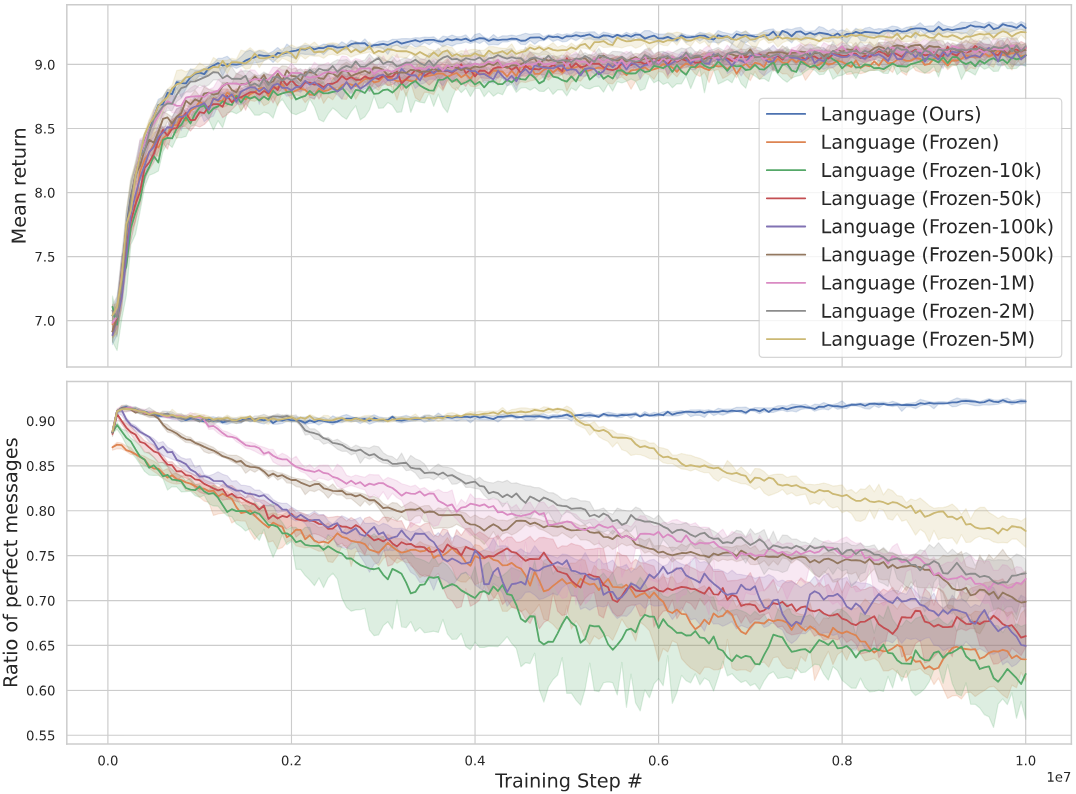
\includegraphics[width=\linewidth]{Figures/LAMAC/AdSA9_15_frzl.png}
    \caption{Effects of stopping language guidance in the fine-tuning experiment (9 runs each, with median and 95\% confidence interval). The top graph shows the task performance across fine-tuning. The bottom graph displays the ratio of generated messages that match the "perfect" description given by the oracle.}
    \label{fig:LAMAC:ad9_15_frzl}
\end{figure}



\subsection{Zero-Shot Teaming}\label{sec:LAMAC:Exp_ZST}

One other aspect of generalisation that is specific to the multi-agent setting is the problem of adapting to new, unknown teammates. Agents trained with a fixed team of partners may overfit their learnt policy to the policies of other agents. This can be a problem if agents are expected to work with new partners during their lifetime, as could be the case in robotic settings. We expect the overfitting problem to be even more problematic when agents are trained with emergent communication, as the emergent language will likely differ between separate teams of agents. On the other hand, language is, by definition, a tool for enabling communication with unknown partners. Thus, language can be helpful to improve zero-shot teams. 

\subsubsection{Protocol}

To evaluate communication strategies in zero-shot teaming, we take the four best teams of each variant after being trained in the $9\times 9$ environment. We then build new teams with agents randomly picked from these four original teams. Each new team is evaluated on 250 episodes of Predator-Prey. The team's evaluation score is the mean of all returns obtained in these episodes. For each agent version, we evaluate one thousand different randomly picked teams and then record the mean and standard deviation of evaluation scores. Table~\ref{tab:LAMAC:ZST} shows these results. To investigate the effect of increasing heterogeneity in teams, we evaluate different team compositions, as shown in the table. The team compositions go from an unmodified team ("AAAA" in the table), used as a baseline, to a fully mixed team with one agent from each pre-trained run ("ABCD"). 

\subsubsection{Results}

Results shown in Table~\ref{tab:LAMAC:ZST} confirm our hypothesis and demonstrate the potential of language for improving zero-shot teaming. As expected, newly formed teams are less efficient in all variants, but language-based ones suffer less from this. \texttt{Emergent-Continuous} agents suffer the most from having to communicate with unknown agents, with performance dropping significantly with only one external agent in the team. Interestingly, the \texttt{Emergent-Discrete} agents suffer less. This may indicate that discrete symbols can be more easily interpreted by unknown agents, or that these agents are less concerned by communication, which is beneficial in this case. Again, a deeper analysis of the emergent language could help clarify the situation. Another interesting observation is that \texttt{Language} agents lose more performance than \texttt{Oracle} ones, showing that the small language imperfections add up in more heterogeneous teams which hinders performance. However, this confirms that communicating with a shared language allows better understanding with unknown partners. 

% \begin{table}[t]
%     \begin{tabular}{cccccc}
%         \hline
%         \small
%                              & \multicolumn{5}{c}{Team Composition}                                    \\ \cline{2-6} 
%         \multicolumn{1}{l}{} & AAAA        & AAAB        & AABB         & AABC         & ABCD          \\ \hline
%         No Comm              & 7.97\pm0.26 & 1.36\pm4.51 & -0.47\pm4.59 & -5.62\pm5.6  & -9.46\pm3.83  \\
%         Em-Continuous        & 8.82\pm0.13 & 1.87\pm4.69 & -1.03\pm5.39 & -6.01\pm5.87 & -13.44\pm4.56 \\
%         Em-Discrete          & 8.19\pm0.23 & 1.62\pm4.71 & 0.99\pm3.75  & -4.38\pm5.92 & -7.97\pm4.45  \\
%         Oracle               & 8.85\pm0.22 & \B 5.08\pm0.22 & \B 4.6\pm2.55   & \B 0.98\pm4.28  & \B -3.22\pm5.43  \\
%         Language             & \B 8.94\pm0.15 & 4.12\pm3.75 & 3.18\pm1.94  & -2.36\pm4.73 & -9.28\pm5.44  \\ \hline
%     \end{tabular}
%     \caption{Zero-shot teaming results (SHOULD BE REPLACED BY RESULTS FROM SA VERSION OF ENV)}
%     \label{tab:LAMAC:ZST}
% \end{table}

\begin{table}[t]
    \centering
    \centerline{\begin{tabular}{cccccc}
        \hline
        \small
                             & \multicolumn{5}{c}{Team Composition}                                    \\ \cline{2-6} 
        \multicolumn{1}{l}{} & AAAA        & AAAB        & AABB         & AABC         & ABCD          \\ \hline
        % No Comm              & $8.71\pm0.13$ & $7.41\pm1.47$ & $6.82\pm1.73$ & $6.69\pm1.29$  & $6.42\pm1.16$  \\
        Em-Continuous        & $7.98\pm0.30$ & $4.63\pm1.78$ & $3.43\pm1.69$ & $2.97\pm1.59$ & $2.49\pm1.42$ \\
        Em-Discrete          & $8.63\pm0.17$ & $6.81\pm1.49$ & $6.15\pm1.7$  & $5.67\pm1.72$ & $5.16\pm1.79$  \\
        Oracle               & $8.93\pm0.19$ & $7.19\pm1.41$ & $6.48\pm1.36$   & $6.35\pm1.38$  & $5.91\pm1.6$  \\
        Language             & $9.06\pm0.1$ & $7.38\pm1.19$ & $6.43\pm1.49$  & $6.06\pm1.67$ & $5.47\pm1.73$  \\ \hline
    \end{tabular}}
    \caption{Results of the zero-shot teaming experiments. New teams are composed from the best four runs of each variant. The scores shown are the mean and standard deviation of one thousand evaluation runs, with one run corresponding to (i) picking agents in pre-trained teams randomly according to the team composition, (ii) running 250 episodes in the $9\times 9$ map, and (iii) record the mean return on these episodes as evaluation score. Increasingly heterogeneous teams are composed to measure the impact of having unknown partners on performance. Letters indicate the team composition: "AAAA" is an unmodified team, "AAAB" has three agents from one run and one agent from another, etc.}
    \label{tab:LAMAC:ZST}
\end{table}

% \begin{table}[t]
%     \begin{tabular}{cccccc}
%         \hline
%         \small
%                              & \multicolumn{5}{c}{Team Composition}                                    \\ \cline{2-6} 
%         \multicolumn{1}{l}{} & AAAA        & AAAB        & AABB         & AABC         & ABCD          \\ \hline
%         No Comm              & $8.85\pm0.11$ & $8.78\pm0.12$ & $8.77\pm0.13$ & $8.74\pm0.13$  & $8.72\pm0.13$  \\
%         Em-Continuous        & $8.89\pm0.11$ & $8.56\pm0.33$ & $8.4\pm0.39$ & $8.31\pm0.36$ & $8.2\pm0.38$ \\
%         Em-Discrete          & $8.73\pm0.12$ & $8.66\pm0.13$ & $8.64\pm0.14$  & $8.62\pm0.14$ & $8.6\pm0.14$  \\
%         Oracle               & $9.26\pm0.2$ & $9.25\pm0.17$ & $9.24\pm0.15$   & $9.25\pm0.12$  & $9.24\pm0.09$  \\
%         Language             & $9.34\pm0.08$ & $9.32\pm0.08$ & $9.3\pm0.08$ & $9.29\pm0.08$ & $9.28\pm0.09$  \\ \hline
%     \end{tabular}
%     \caption{Zero-shot teaming results $15\times 15$}
%     \label{tab:LAMAC:ZST}
% \end{table}

% \subsection{Interpretation}\label{sec:LAMAC:Exp_Interpret}

% % Put this in the "Learning to communicate" ? (-> "we successively learn language communication")
% % \subsubsection{Protocol}

% % \subsubsection{Results}

% E


\subsection{Interaction}\label{sec:LAMAC:Exp_Interact}

A desired feature for communicating agents is the possibility of interacting with them. If the agents' communication system is interpretable, then we can try using this system for interaction. Making agents learn a language we designed solves the issue of interpretability and should make interaction straightforward. To evaluate this quantitatively, we investigate the impact of human messages on the agents' behaviour. 

% FIGURE Interaction
\begin{figure}
    \centering
    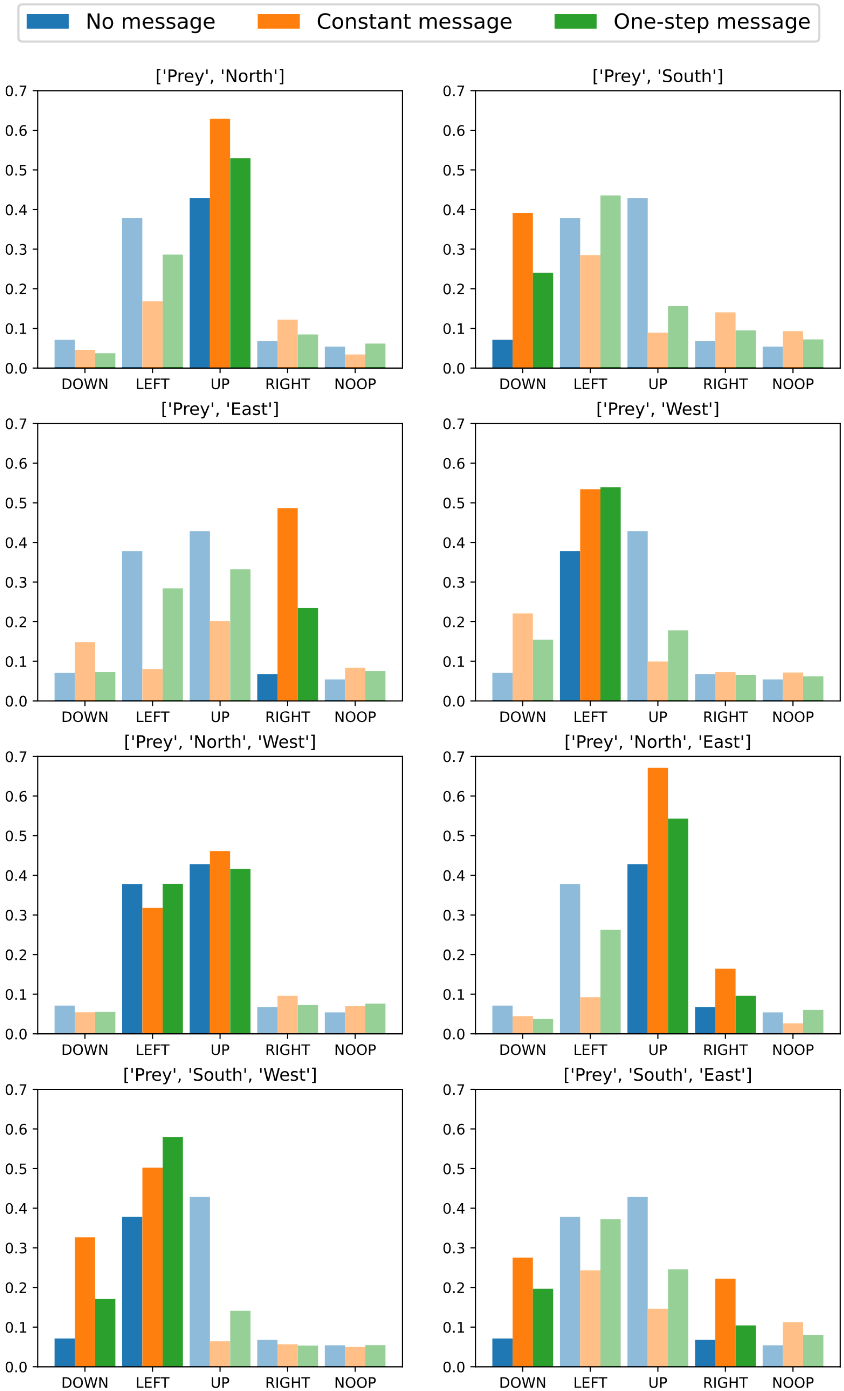
\includegraphics[width=0.92\linewidth]{Figures/LAMAC/interact.png}
    \caption{Results of the interaction experiments. Each plot shows the impact of the corresponding messages on action probabilities. "No message" is a control group that receives no message (same for all graphs). "Constant message" receives the message at every step. "One-step message" receives it only on the first step. The highlighted bars correspond to the direction that should be favoured given the input message.}
    \label{fig:LAMAC:interact}
\end{figure}

\subsubsection{Protocol}

To measure this, we put a pre-trained team of \texttt{Language} agents in an empty environment, send a message into the communication channel, and record the actions performed in the following 5 steps. Agents are spawned in central positions and provided a message indicating that a prey is located in one region of the environment. We execute these short episodes a large number of times and record the performed actions. In Figure~\ref{fig:LAMAC:interact}, we display the observed probabilities of each action following the given messages. We compare the action probabilities for agents receiving no message ("No messages"), agents constantly receiving the messages during 5 steps ("Constant message"), and agents that receive the message on the first step and no message during the four remaining steps ("One-step message"). The latter can be indicative of the good use of memory by the agents. 

We found that four-agent teams are difficult to evaluate this way because they tend to have different agents focusing on the four corners of the map. Thus, regardless of the input message, action probabilities will balance themselves. Therefore, we train a team of two \texttt{Language} agents in the $15\times 15$ map and evaluate them. Because these two agents need to catch preys together, their average action probabilities should be impacted by the input messages. The larger map size will help increase the contribution of communication over exploration. 

\subsubsection{Results}

Looking at the graph of Figure~\ref{fig:LAMAC:interact}, we find that messages almost always impact the agents' behaviour accordingly. Only the "Prey North West" message has no clear impact, which may be linked to the fact that these agents seem to be biased toward the "LEFT" and "UP" actions, as seen in the control group. For all other messages, the corresponding action probabilities are significantly increased. Even the "One-step message" impacts the agents' actions, showing that agents have learnt to memorise previously received messages. Overall, it is clear that we can impact the behaviour of \texttt{Language} agents by communicating with them.














% -------------------------------------------------------------------------------------------------

\section{Discussions}

\subsection{Analysing and Discussing Results}\label{sec:LAMAC:Discuss_Results}

With this set of experiments, we have shown that:
\begin{itemize}
    \item \textbf{Agents successively learn to use a language} that describes their observations, concurrently to learning an embodied multi-agent task. 
    \item \textbf{Language improves communication}. Agents using language learn faster than the ones learning emergent communication. This seems natural, as agents are given an efficient communication system and are trained to not deviate from it. They do not experience the struggle of finding a consensus on how to communicate, while also learning a policy. Thus, language-based communication makes training more stable. 
    \item \textbf{Learning language allows faster learning} by guiding the learning of efficient representation. By learning language, agents (i) ground their representations of the observation space in concepts expressed in language and (ii) ground their representations of language messages in their knowledge of the observation space.
    \item \textbf{Using a pre-defined language grants multiple desired features} to our agents: better adaptation to new environments or partners, interpretability, and interaction. 
\end{itemize}

Of course, all these advantages brought by language come at the cost of providing the supervision required for learning this language. In our case, the cost is two-fold. First, we need the oracle to generate the language descriptions used for learning language. Relying on such rule-based systems restricts us to simple environments with relatively poor language structures. This is not necessarily an issue: simple robotic tasks might not benefit from using more complex languages. However, if more complex tasks are envisioned, more capable techniques may be required. In the robotic setting, for instance, many recent works have provided datasets~\citep{Nair2021_LORL} and models~\citep{Zeng2022_Socratic} for captioning images related to robot behaviour. Second, we pay the cost of training and using language-based tools. The sequenced structure of language makes its processing quite slow. In our case, learning to communicate with language has doubled the training time compared to the continuous emergent communication variant. We still consider that the gains of language-based agents, in their understanding of the world and communication skills, can justify these costs. However, it would still be beneficial to try reducing them. In the next section, we provide some avenues of improvement for better language learning.
%that we will implement in future works. 
% all these advantages come at a cost
% - need data: for us it's the parser, however real world settings could benefit from captioning models that can describe various situations from pictures
% - takes time: encode/generate sentences
% but no cost at all for the post-mortem qualities showed (interaction, zst)
% lower cost for generalisation

About the emergent communication baseline that we define, it is important to note that they could be improved in many ways, as shown in the extensive related literature (see Section~\ref{sec:MADRL:EmergentCommunication} and ~\ref{sec:LAMAC:RW_Grouding}). Our point is not to say that emergent communication does not work, nor that it has no use. Rather, we want to show that, for robotic-like settings, it fails to fit the requirements on multiple points: interpretability, generalisation, and interaction. Improving emergent communication on these points is possible but will have an important cost with no guaranteed perfect solution. This cost might as well be paid for learning a language that improves communication, grounds representation learning, and provides many desired features to our agents. 

Lastly, to improve our comparison with emergent communication and back our claims further, we could benefit from extending our experiments and analysis of the different communication systems. Experimenting in a more complex setting with more diverse entities and objects could highlight the advantages of learning a pre-defined language further. Additionally, improving our analysis of the learnt communication mechanisms, by measuring the informational content of messages and their impact on other agents~\citep{Lowe2019_Pitfalls, Jaques2019_SocialInfluence}, would be helpful to better showcase the shortcomings of emergent communication systems and the qualities of pre-defined languages.




% Bandwidth comparison between different communication strategies

% - EmComm could be better, we implement a simple version, previous works have devised techniques to make emergent communication better.
% - but they require a lot of care to design and make work, only to have a black box communication protocol at the end
% - we want to show that learning to communicate with language in an embodied setting is possible and has many advantages

% - to improve comparison, we could benefit from reproducing these experiments in other settings that feature a larger diversity of entities/objects, thus more complex language
% - improving our analysis of emergent communication can also help reveal its shortcomings

% \subsection{Learning results: costs and benefits}\label{sec:LAMAC:Discuss_Language}


\subsection{Perspectives for Improving Language Learning}\label{sec:LAMAC:Discuss_LangImprov}

Our implementation of language learning has one flaw that increases its costs substantially: it does not exploit the acquired language examples sufficiently. The data used for training on the language objectives is the same as the one used for training PPO, i.e., we use only the data gathered between each training phase to train the language modules. A more sensible approach would be to build a dataset of language examples throughout training, without discarding data after the training phase. This could improve language learning by training on more diverse data. Importantly, this would allow limiting the cost of annotation by limiting the number of calls to the oracle. As in the generalisation experiment (see Section~\ref{sec:LAMAC:Exp_Generalisation}), we could stop the generation of language examples after a given number of training steps, but continue training on the language objectives indefinitely using the buffered language examples. This would prevent the loss of language quality observed in the "frozen" agents in Figure~\ref{fig:LAMAC:ad9_15_frzl}. 

Another way of improving language learning would be to use more advanced techniques for the language modules. In our architecture, we use one-layer GRUs and small MLPs for these modules. In other words, we use the most basic neural networks possible for implementing the language modelling skills. This is largely sufficient for learning a simple language like the one we have. But, more complex techniques like deeper neural networks or Transformers would improve language learning and allow learning more complex languages. 
% study of comm eps: show if it has impact on language learning, can other values improve learning (especially in the generalisation setting)

% \subsection{Positioning related to LLM-agents}\label{sec:LAMAC:Discuss_LLMs}

% As reviewed in Section~\ref{sec:LAMAC:RW_NaturalLang}, many recent works have proposed interesting ways of using LLMs for handling reasoning and communication in multi-agent and robotic settings~\citep{Carta2023_GLAM, Driess2023_PaLME, Li2023_ToMLLM, Liu2024_HLA, Zhang2024_CoELA, Zhu2024_CognitiveLLMs}. While these approaches have some interesting potential for studying high-level social interactions, ththey may suffer from known issues of LLMs  
% we want to show that it is possible to learn language with a rather small architecture. we don't need a LLM to learn a simple language. We don't need a complicated language to perform simple robotic tasks: it would be unnecessary to teach a box pushing robot how to speak English fluently. Thus, we can make concessions and allow smaller, more compute-efficient agent architectures. 
% that said, the idea and algorithms proposed are agnostic to any particular neural architecture. we could scale the full architecture to use Transformers or even LLMs, to fit the needs of more complicated tasks, with more complicated languages. But, we believe that (an important part of this work is to show the importance) of grounding language understanding in observations, and conversely ground action-selection in language. This enables learning the language fully, not only by learning how symbols should be associated \footnote{See the Chinese room argument that can be used to challenge language modelling [Harnad1990]},  but also by understanding the meanings behind symbol associations in terms of environmental situations. This can only be achieved by learning language while learning to behave in the environment. Using a pre-trained LLM would not allow this to happen and, thus, would [fail to capture true language-understanding, in the embodied sense]

% problems of LLMs 
% - not perfect with language Mahowald2024_LLMLangThought

\subsection{Conclusion and Future Works}\label{sec:LAMAC:Discuss_FuturWorks}

To conclude, in this chapter, we have proposed a method for enabling embodied agents to learn a pre-defined language while training on a cooperative task with MADRL. By learning this language, agents gain the ability to communicate efficiently about their local observations, as the language has been purposefully designed to express meanings that serve the task at hand. Additionally, agents can exploit the structures in the given language to ground their understanding of the world, allowing more efficient representation learning. In addition to these learning improvements, training language-augmented agents also presents multiple practical advantages. Because communication is carried out in a known language, interpreting the communication acts is straightforward. This works in the other way, with agents being able to receive information from human experimenters. Language-augmented agents are also able to better generalise their knowledge, enabling faster adaptation to changes in the environment. Lastly, language-based communication enables easier cooperation with unknown partners, by providing a shared communication system to support social interactions. 

With this work, we showcase the great potential of language-augmented agents for the multi-agent setting. This should encourage further works on this subject to explore this potential in more depth. In future works, we will study ways to expand the language capabilities of our agents. As human beings, artificial agents would benefit from sharing their intentions with their partners. Taking inspiration from works in language-augmented, goal-driven learning, we could extend our architecture to allow agents to communicate about intents. Another area for improvement is the diversity of communicating behaviours. Fine-tuning language modules with RL could allow more diverse communication strategies. Finally, the generalisation abilities of language-grounded agents are particularly interesting. As a single language can describe similar situations in completely different environments, it can support the transfer of a learnt policy to new domains, by grounding different state spaces in common linguistic concepts. This could help to drastically reduce the cost of learning multi-agent strategies in realistic robotic domains. 
% good results

% many oportunities for scaling and improvements

% - sharing intents (need goal conditioning): captioning a sequence of time-steps that can be associated with an action description
% - different ways of sharing messages (not broadcasts)
% - training the communication policy with RL to enable more learnt communication behaviour, but still based on the language background given to agents
% - sim to sim, sim to real
% - scaling to more complex environments (more and more datasets are produce to learn visual language alignment in robotic settings, or use LLM to caption a robots observations during training)
